
\documentclass[a4paper,twoside,12pt]{book}
\usepackage[utf8]{inputenc}                                      
\usepackage[T1]{fontenc}  
\usepackage{amsmath,amsfonts,amssymb,amsthm}
\usepackage[british,polish]{babel} 
\usepackage{indentfirst}
\usepackage{lmodern}
\usepackage{graphicx} 
\usepackage{hyperref}
\usepackage{booktabs}
%\usepackage{tikz}
%\usepackage{pgfplots}
\usepackage{mathtools}
\usepackage{geometry}
\usepackage[page]{appendix} % toc,
\renewcommand{\appendixtocname}{Dodatki}
\renewcommand{\appendixpagename}{Dodatki}
\renewcommand{\appendixname}{Dodatek}

\usepackage{setspace}
\onehalfspacing


\frenchspacing

\usepackage{listings}
%\lstset{
%	language={},
%	basicstyle=\ttfamily,
%	keywordstyle=\lst@ifdisplaystyle\color{blue}\fi,
%	commentstyle=\color{gray}
%}

%%%%%%%%%%%%%%%%%%%%%%%%%%%
% listingi 
\usepackage{listings}
\lstset{%
language=C++,%
commentstyle=\textit,%
identifierstyle=\textsf,%
keywordstyle=\sffamily\bfseries, %\texttt, %
%captionpos=b,%
tabsize=3,%
frame=lines,%
numbers=left,%
numberstyle=\tiny,%
numbersep=5pt,%
breaklines=true,%
morekeywords={descriptor_gaussian,descriptor,partition,fcm_possibilistic,dataset,my_exception,exception,std,vector},%
escapeinside={@*}{*@},%
%texcl=true, % wylacza tryb verbatim w komentarzach jednolinijkowych
}
%%%%%%%%%%%%%%%%%%%%%%%%%%%%%%%%%%%%


%%%%%%%%%

%%%% TODO LIST GENERATOR %%%%%%%%%

%\usepackage{tikz}
%\usepackage{manfnt}   % dangerous sign 
\usepackage{color}
\definecolor{brickred}      {cmyk}{0   , 0.89, 0.94, 0.28}

\makeatletter \newcommand \kslistofremarks{\section*{Uwagi} \@starttoc{rks}}
  \newcommand\l@uwagas[2]
    {\par\noindent \textbf{#2:} %\parbox{10cm}
{#1}\par} \makeatother


\newcommand{\ksremark}[1]{%
{%\marginpar{\textdbend}
{\color{brickred}{[#1]}}}%
\addcontentsline{rks}{uwagas}{\protect{#1}}%
}

\newcommand{\comma}{\ksremark{przecinek}}
\newcommand{\nocomma}{\ksremark{bez przecinka}}
\newcommand{\styl}{\ksremark{styl}}
\newcommand{\ortografia}{\ksremark{ortografia}}
\newcommand{\fleksja}{\ksremark{fleksja}}
\newcommand{\pauza}{\ksremark{pauza `--', nie dywiz `-'}}
\newcommand{\kolokwializm}{\ksremark{kolokwializm}}

%%%%%%%%%%%%%% END OF TODO LIST GENERATOR %%%%%%%%%%%

%%%%%%%%%%%% ZYWA PAGINA %%%%%%%%%%%%%%%
% brak kapitalizacji zywej paginy
\usepackage{fancyhdr}
\pagestyle{fancy}
\fancyhf{}
\fancyhead[LO]{\nouppercase{\it\rightmark}}
\fancyhead[RE]{\nouppercase{\it\leftmark}}
\fancyhead[LE,RO]{\it\thepage}


\fancypagestyle{tylkoNumeryStron}{%
   \fancyhf{} 
   \fancyhead[LE,RO]{\it\thepage}
}

\fancypagestyle{NumeryStronNazwyRozdzialow}{%
   \fancyhf{} 
   \fancyhead[LO]{\nouppercase{\it\rightmark}}
   \fancyhead[RE]{\nouppercase{\it\leftmark}}
   \fancyhead[LE,RO]{\it\thepage}
}


%%%%%%%%%%%%% OBCE WTRETY  
\newcommand{\obcy}[1]{\emph{#1}}
\newcommand{\ang}[1]{{\selectlanguage{british}\obcy{#1}}}
%%%%%%%%%%%%%%%%%%%%%%%%%%%%%

% polskie oznaczenia funkcji matematycznych
\renewcommand{\tan}{\operatorname {tg}}
\renewcommand{\log}{\operatorname {lg}}

% jeszcze jakies drobiazgi

\newcounter{stronyPozaNumeracja}

\newcommand{\hcancel}[1]{%
    \tikz[baseline=(tocancel.base)]{
        \node[inner sep=0pt,outer sep=0pt] (tocancel) {#1};
        \draw[red] (tocancel.south west) -- (tocancel.north east);
    }%
}%

\newcommand{\miesiac}{%
  \ifcase\the\month
  \or styczeń% 1
  \or luty% 2
  \or marzec% 3
  \or kwiecień% 4
  \or maj% 5
  \or czerwiec% 6
  \or lipiec% 7
  \or sierpień% 8
  \or wrzesień% 9
  \or październik% 10
  \or listopad% 11
  \or grudzień% 12
  \fi}


%%%%%%%%%%%%%%%%%%%%%%%%%%%%%%%%%%%%%%%%%%%%%%
% Helvetica font macros for the title page:
\newcommand{\headerfont}{\fontfamily{phv}\fontsize{18}{18}\bfseries\scshape\selectfont}
\newcommand{\titlefont}{\fontfamily{phv}\fontsize{18}{18}\selectfont}
\newcommand{\otherfont}{\fontfamily{phv}\fontsize{14}{14}\selectfont}

%%%%%%%%%%%%%%%%%%%%%%%%%%%%%%%%%%%%%%%%%%%%%%
%%%%%%%%%%%%%%%%%%%%%%%%%%%%%%%%%%%%%%%%%%%%%%
%%%%%%%%%%%%%%%%%%%%%%%%%%%%%%%%%%%%%%%%%%%%%%
%%%%%%%%%%%%%%%%%%%%%%%%%%%%%%%%%%%%%%%%%%%%%%
%%%%%%%%%%%%%%%%%%%%%%%%%%%%%%%%%%%%%%%%%%%%%%
%%%%%%%%%%%%%%%%%%%%%%%%%%%%%%%%%%%%%%%%%%%%%%
%%%%%%%%%%%%%%%%%%%%%%%%%%%%%%%%%%%%%%%%%%%%%%


\newcommand{\autor}{Seweryn Gładysz}
\newcommand{\promotor}{dr inż. Ewa Płuciennik}
\newcommand{\konsultant}{dr inż. Imię Nazwisko}
\newcommand{\tytul}{System zarządzania siecią siłowni oparty o bazę dokumentową}
\newcommand{\polsl}{Politechnika Śląska}
\newcommand{\wydzial}{Wydział Automatyki, Elektroniki i Informatyki}
\newcommand{\kierunek}{Kierunek: Informatyka}


\begin{document}
%\kslistofremarks 
	
%%%%%%%%%%%%%%%%%%  STRONA TYTULOWA %%%%%%%%%%%%%%%%%%%
\pagestyle{empty}
{
	\newgeometry{top=2.5cm,%
	             bottom=2.5cm,%
	             left=3cm,
	             right=2.5cm}
	\sffamily
	\rule{0cm}{0cm}
	
	\begin{center}
	
\includegraphics[width=29mm]{logo_pl.jpg}
	\end{center} 
	\vspace{1cm}
	\begin{center}
	\headerfont \polsl
	\end{center}
	\begin{center}
	\headerfont \wydzial
	\end{center}
	\begin{center}
	\headerfont \kierunek
	\end{center}
	\vfill
	\begin{center}
	\titlefont Praca dyplomowa inżynierska
	\end{center}
	\vfill
	
	\begin{center}
	\otherfont \tytul\par
	\end{center}
	
	\vfill
	
	\vfill
	 
	\noindent\vbox
	{
		\hbox{\otherfont autor: \autor}
		\vspace{12pt}
		\hbox{\otherfont kierujący pracą: \promotor}
		\vspace{12pt}  % zakomentuj, jezeli nie ma konsultanta
		\hbox{\otherfont konsultant: \konsultant} % zakomentuj, jezeli nie ma konsultanta
	}
	\vfill 
 
   \begin{center}
   \otherfont Gliwice,  \miesiac\ \the\year
   \end{center}	
	\restoregeometry
}
  

\cleardoublepage
 

\rmfamily
\normalfont


%%%%%%%%%%%%%%%%%% SPIS TRESCI %%%%%%%%%%%%%%%%%%%%%%
\pagenumbering{Roman}
\pagestyle{tylkoNumeryStron}
\tableofcontents

%%%%%%%%%%%%%%%%%%%%%%%%%%%%%%%%%%%%%%%%%%%%%%%%%%%%%
\setcounter{stronyPozaNumeracja}{\value{page}}
\mainmatter
\pagestyle{empty}

\chapter*{Streszczenie}

Streszczenie pracy -odpowiednie pole w systemie APD powinno zawierac kopie tego streszczenia. Streszczenie, wraz ze slowami kluczowymi, nie powinno przekroczyc jednej strony.

{\bf Slowa kluczowe:} 2-5 slow (fraz) kluczowych, oddzielonych przecinkami

\addcontentsline{toc}{chapter}{Streszczenie}

\cleardoublepage

\pagestyle{NumeryStronNazwyRozdzialow}

%%%%%%%%%%%%%% wlasciwa tresc pracy %%%%%%%%%%%%%%%%%

\chapter{Wstęp}

\begin{itemize}
\item wprowadzenie w problem/zagadnienie
\item osadzenie problemu w dziedzinie
\item cel pracy
\item zakres pracy
\item zwięzła charakterystyka rozdziałów
\item jednoznaczne określenie wkładu autora, w przypadku prac wieloosobowych – tabela z autorstwem poszczególnych elementów pracy
\end{itemize}

\chapter{Analiza tematu}

Na rynku siłowni widać coraz większą konkurencję, a właściciele szukają sposobów jak zachęcić nowych klientów do uczęszczania na ich siłownie. Wiele z sieci pozwala na całodobowe korzystanie z ich obiektów, aby sprostać wymaganiom jak największej grupie klientów. Stawia to nowe wyzwania w organizacji pracy pracowników i sposobie działania obiektów. Dużym usprawnieniem byłaby możliwość zrezygnowania z recepcji na rzecz bramek wejściowych i wyjściowych, które kontrolowałby ważność karnetu oraz pilnowałby, aby w tej samej chwili na siłowni nie znajdowała się zbyt duża liczba osób.

Innym problemem jest coraz większa liczba sieci siłowni, która w swojej ofercie zawiera możliwość udziału w wydarzeniach grupowych, które pozwalają na uczestnictwo w grupowej sesji, gdzie pracownik siłowni nadzoruje czy uczestnicy wykonują ćwiczenia w sposób bezpieczny dla ich zdrowia. Pozwolenie na zgłoszenie chęci udziału w takim wydarzeniu poprzez aplikacje internetową może zwiększyć atrakcyjność oferty danej sieci siłowni w obliczu rosnącej konkurencji na rynku sieci siłowni.

Sieć siłowni staje w obliczu innych wyzwań, które nie są znane małym sieciom siłowni lub pojedynczym obiektom. Zarządzanie wyposażeniem może być utrudnione ze względu na liczbę posiadanych urządzeń i liczbę obiektów siłowni należących do sieci. System powinien gromadzić informacje na temat posiadanego sprzętu, aby skrócić czas, jaki jest potrzebny to przeprowadzenia inwentaryzacji posiadanych akcesoriów i sprzętów do ćwiczeń.

Innym wyzwaniem stawianym przed właścicielami siłowni jest stworzenie oferty treningów personalnych dla klientów, którzy oczekują indywidualnego podejścia do treningu. Rozwiązaniem jest stworzenie modułu, który pozwalałby na rezerwowanie przez klientów terminów treningów. Takie rozwiązanie może zwiększyć atrakcyjność danej sieci oraz pozwolić na sprawniejsze organizowanie czasu trenerów personalnych należących do sieci siłowni.

Ważnym wyzwaniem stawianym przez pandemię koronawirusa jest reagowanie na częste zmiany w przepisach dotyczących wstępu na obiekty sportowe. Taka sytuacja zmusza właścicieli do ciągłego monitorowania sytuacji i reagowania na zmiany dotyczące przepisów sanitarnych. Każda taka zmiana zmusza siłownię do wdrożenia nowych restrykcji w postaci limitów osób na siłowni. Pomocą w realizowaniu narzuconych obostrzeń byłoby stworzenie systemu, który ustalałby jaka jest maksymalna liczba osób w obiekcie na podstawie wprowadzonych danych. System powinien również zapewniać możliwość kontrolowania liczby osób, które znajdują się w danej chwili w obiekcie siłowni.

Kolejnym problemem jest ilość użytkowników korzystających z system informatycznego. Sieć siłowni w przeciwieństwie do pojedynczego obiektu musi obsługiwać żądania dużej liczby klientów. Aby zapewnić ciągłość działania systemu ważne jest aby stworzone oprogramowanie było skalowalne. Skalowanie może zostać wykonywane \textit{w górę} (poprzez zmodyfikowanie serwera w celu poprawy jego wydajności) lub \textit{w szerz} (rozdzielenie obciążenia pomiędzy większą liczbą serwerów)\footnote{\cite{bib:mongodb_guide}}. W wielu przypadkach skalowanie w górę jest zbyt kosztowne lub niemożliwe ze względu na ograniczenia technologiczne. W takim przypadku z pomocą przychodzi skalowanie wszerz, które pozwala na rozdzielenie obciążenia pomiędzy różnymi maszynami.

Aktualnie w sieci Internet możemy znaleźć wiele dostępnych rozwiązań, które pokrywają wymagania funkcjonalne systemu. Duża część oferowanych aplikacji posiada możliwość zarządzania bazą klientów, prowadzenie inwentarza wyposażenia oraz opcję tworzenia bogatej oferty karnetów. Największe aplikacje posiadają w swoim zakresie funkcjonalnym rozwiązania wymienionych problemów, jednak żadne z nich nie posiada modułu odpowiedzialnego za zarządzanie dostępem do siłowni pod kątem obowiązujących przepisów sanitarnych. W celu zaproponowania systemu informatycznego, który będzie konkurencyjny na rynku, system powinien posiadać taki moduł.

Tworzony system powinien zapewnić wsparcie pracownikom w spełnianiu aktualnych norm i obostrzeń sanitarnych oraz dostarczyć podstawowe funkcjonalności potrzebne w prowadzeniu działalności sieci siłowni. W celu uniknięcia problemów z wydajnością, a tym samym złym doświadczeniom płynącym z korzystania z serwisu internetowego, system musi być podatny na zmiany. Aplikacja powinna cechować się skalowalnością w celu zapewnienia szybkości działania nawet w przypadku dużej liczby aktywnych użytkowników. Aby to osiągnąć system powinien zostać utworzony przy pomocy infrastruktury, która pozwoli na skalowanie wszerz. Warstwa serwerowa aplikacji powinna zostać utworzona w technologii i przy pomocy metodyk, które pozwolą na łatwe dostosowanie aplikacji do architektury mikro-usług.

\chapter{Wymagania i narzędzia}

\begin{itemize}
	\item Wymagania funkcjonalne
	\\ Wymienione punkty stanowią listę wszystkich funkcjonalności jakie powinna oferować aplikacja. Opisują one jakie funkcje  zostały udostępnione użytkownikowi poprzez warstwę prezentacji oraz interfejs REST API.
		\begin{itemize}
			\item Tworzenie konta trenera personalnego - w systemie powinna istnieć możliwość dodawania kont, dla pracowników siłowni w celu zarządzania zasobami siłowni.
			\item Rejestracja konta klienta - system powinien pozwalać na samodzielne zarejestrowanie się użytkownika w celu skorzystania z funkcjonalności serwisu internetowego sieci siłowni.
			\item Logowanie się na wcześniej utworzone konto użytkownika - w celu weryfikacji użytkownika, system powinien pozwalać na autoryzację poprzez formularz logowania.
			\item Przeglądanie dostępnej oferty karnetów na siłownie - użytkownik w celu zakupu karnetu musi mieć możliwość przeglądania dostępnej oferty.
			\item Przedłużenie karnetu przypisanego do konta użytkownika - użytkownik posiadający już karnet może go przedłużyć.
			\item Zakup karnetu - użytkownik, powinien mieć możliwość zakupu karnetu w celu wejścia do siłowni.
			\item Utworzenie nowego typu karnetu - pracownicy siłowni powinni mieć możliwość stworzenia oferty karnetów.
			\item Usunięcie istniejącego rodzaju karnetu - pracownicy siłowni powinni mieć możliwość usunięcia z oferty wcześniej utworzonych karnetów.
			\item Edycja istniejącego typu karnetu - pracownicy siłowni powinni mieć możliwość dokonania zmian w istniejącej ofercie karnetów.
			\item Edycja informacji o koncie użytkownika - użytkownik serwisu powinien mieć możliwość edycji informacji zawartych w swoim profilu.
			\item Archiwizacja konta użytkownika - użytkownik serwisu powinien mieć możliwość zarchiwizowania swojego konta, gdy nie jest już zainteresowany dalszym korzystaniem z serwisu.
			\item Przeglądanie listy dostępny wydarzeń - użytkownicy powinni mieć możliwość przeglądania listy dostępnych wydarzeń.
			\item Utworzenie nowego wydarzenia - trenerzy personalni powinni mieć możliwość dodawania wydarzeń, które będą miały miejsce na terenie siłowni.
			\item Odwołanie wydarzenia - trener personalny powinien mieć możliwość odwołania zaplanowanego wydarzenia.
			\item Edycja wydarzenia - trener personalny powinien mieć możliwość wprowadzenia zmian w zaplanowanym wydarzeniu.
			\item Możliwość zapisania się na udział w wydarzeniu - klient powinien mieć możliwość zdeklarowania chęci udziału w wydarzeniu.
			\item Rezygnacja z udziału w wydarzeniu - klient powinien mieć możliwość zrezygnowania z udziału w wydarzeniu, w którym wcześniej zdeklarował chęć udziału.
			\item Utworzenie nowego obiektu siłowni - pracownicy powinni mieć możliwość utworzenia nowych obiektów sieci siłowni.
			\item Możliwość zdefiniowania ograniczeń dostępu do siłowni - pracownicy powinni mieć możliwość zdefiniowania limitu osób jaki może się znajdować w obiekcie siłowni.
			\item Możliwość dodania nowych pomieszczeń dla obiektu siłowni - pracownicy powinni mieć możliwość dodania nowych pomieszczeń do obiektu siłowni.
			\item Możliwość usunięcia pomieszczeń z obiektu siłowni - pracownicy powinni mieć możliwość usunięcia pomieszczenia, które zostało utworzone w danym obiekcie siłowni.
			\item Możliwość zdefiniowania akcesoriów i sprzętu do ćwiczeń - pracownicy powinni mieć możliwość zdefiniowania akcesoriów dostępnych w danym obiekcie siłowni.
			\item Edycja zdefiniowanych akcesoriów i sprzętu do ćwiczeń - pracownicy powinni mieć możliwość edycji wcześniej zdefiniowanych akcesoriów i sprzętu do ćwiczeń.
			\item Możliwość uruchomienia aplikacji w trybie bramki wejściowej - aplikacja powinna pozwolić użytkownikowi na uruchomienie aplikacji w trybie bramki wejściowej w celu kontroli liczby klientów znajdujących się w siłowni.
			\item Możliwość uruchomienia aplikacji w trybie bramki wyjściowej - aplikacja powinna pozwolić użytkownikowi na uruchomienie aplikacji w trybie bramki wyjściowej w celu kontroli liczby klientów wychodzących z siłowni.
			\item Przeglądanie listy dostępnych treningów indywidualnych - użytkownicy powinni mieć możliwość przeglądania listy dostępnych treningów osobisty.
			\item Możliwość zapisania się na udział w treningu indywidualnym - klient powinien mieć możliwość zapisania się na wcześniej utworzony trening indywidualny z trenerem personalnym.
			\item Utworzenie treningu indywidualnego - trener personalny powinien mieć możliwość utworzenia sesji treningów indywidualnych.
			\item Odwołanie treningu indywidualnego - trener personalny powinien mieć możliwość odwołania wcześniej zaplanowanych treningów personalnych.
			\item Rezygnacja z udziału w treningu personalnym - klient powinien mieć możliwość zrezygnowania z udziału w treningu personalnym.
			\item Odmowa wejścia na siłownie - bramka wejściowa powinna mieć możliwość odmówienia wejścia klientowi na siłownie w przypadku braku ważnego karnetu lub osiągnięciu maksymalnej liczby klientów na terenie obiektu siłowni.
			\item Sprawdzenie czy jest możliwość wejścia na siłownię - bramka wejściowa powinna informować o limicie osób, jaki może znajdować się w obiekcie siłowni.
			\item Otwarcie bramki wejściowej - bramka wejściowa powinna pozwolić na wejście na teren siłowni po spełnieniu warunków.
			\item Otwarcie bramki wyjściowej - bramka wyjściowa powinna pozwolić na wyjście z terenu siłowni.
		\end{itemize}
			
	\item Wymagania niefunkcjonalne
		\begin {itemize}
			\item Wyświetlanie elementów interfejsu użytkownika powinno zostać dostosowane do standardowych rozdzielczości ekranów komputerów osobistych.
			\item Poprawny sposób działania w nowoczesnych przeglądarkach: Mozilla Firefox, Google Chrome, Microsoft Edge.
			\item System powinien pozwolić na obsłużenie równoczesnego dostępu do aplikacji dla co najmniej stu użytkowników równocześnie.
			\item Aplikacja powinna być dostępna dla użytkowników przez siedem dni w tygodniu w godzinach 3-22.
		\end{itemize}
	
	\item Diagram przypadków użycia (UML)
	\\ Diagram przypadków użycia pozwala na przedstawienie interakcji użytkowników z aplikacją i przedstawienie wymogów funkcjonalnych systemu w formie diagramów.
	
\begin{figure}
	\centering
	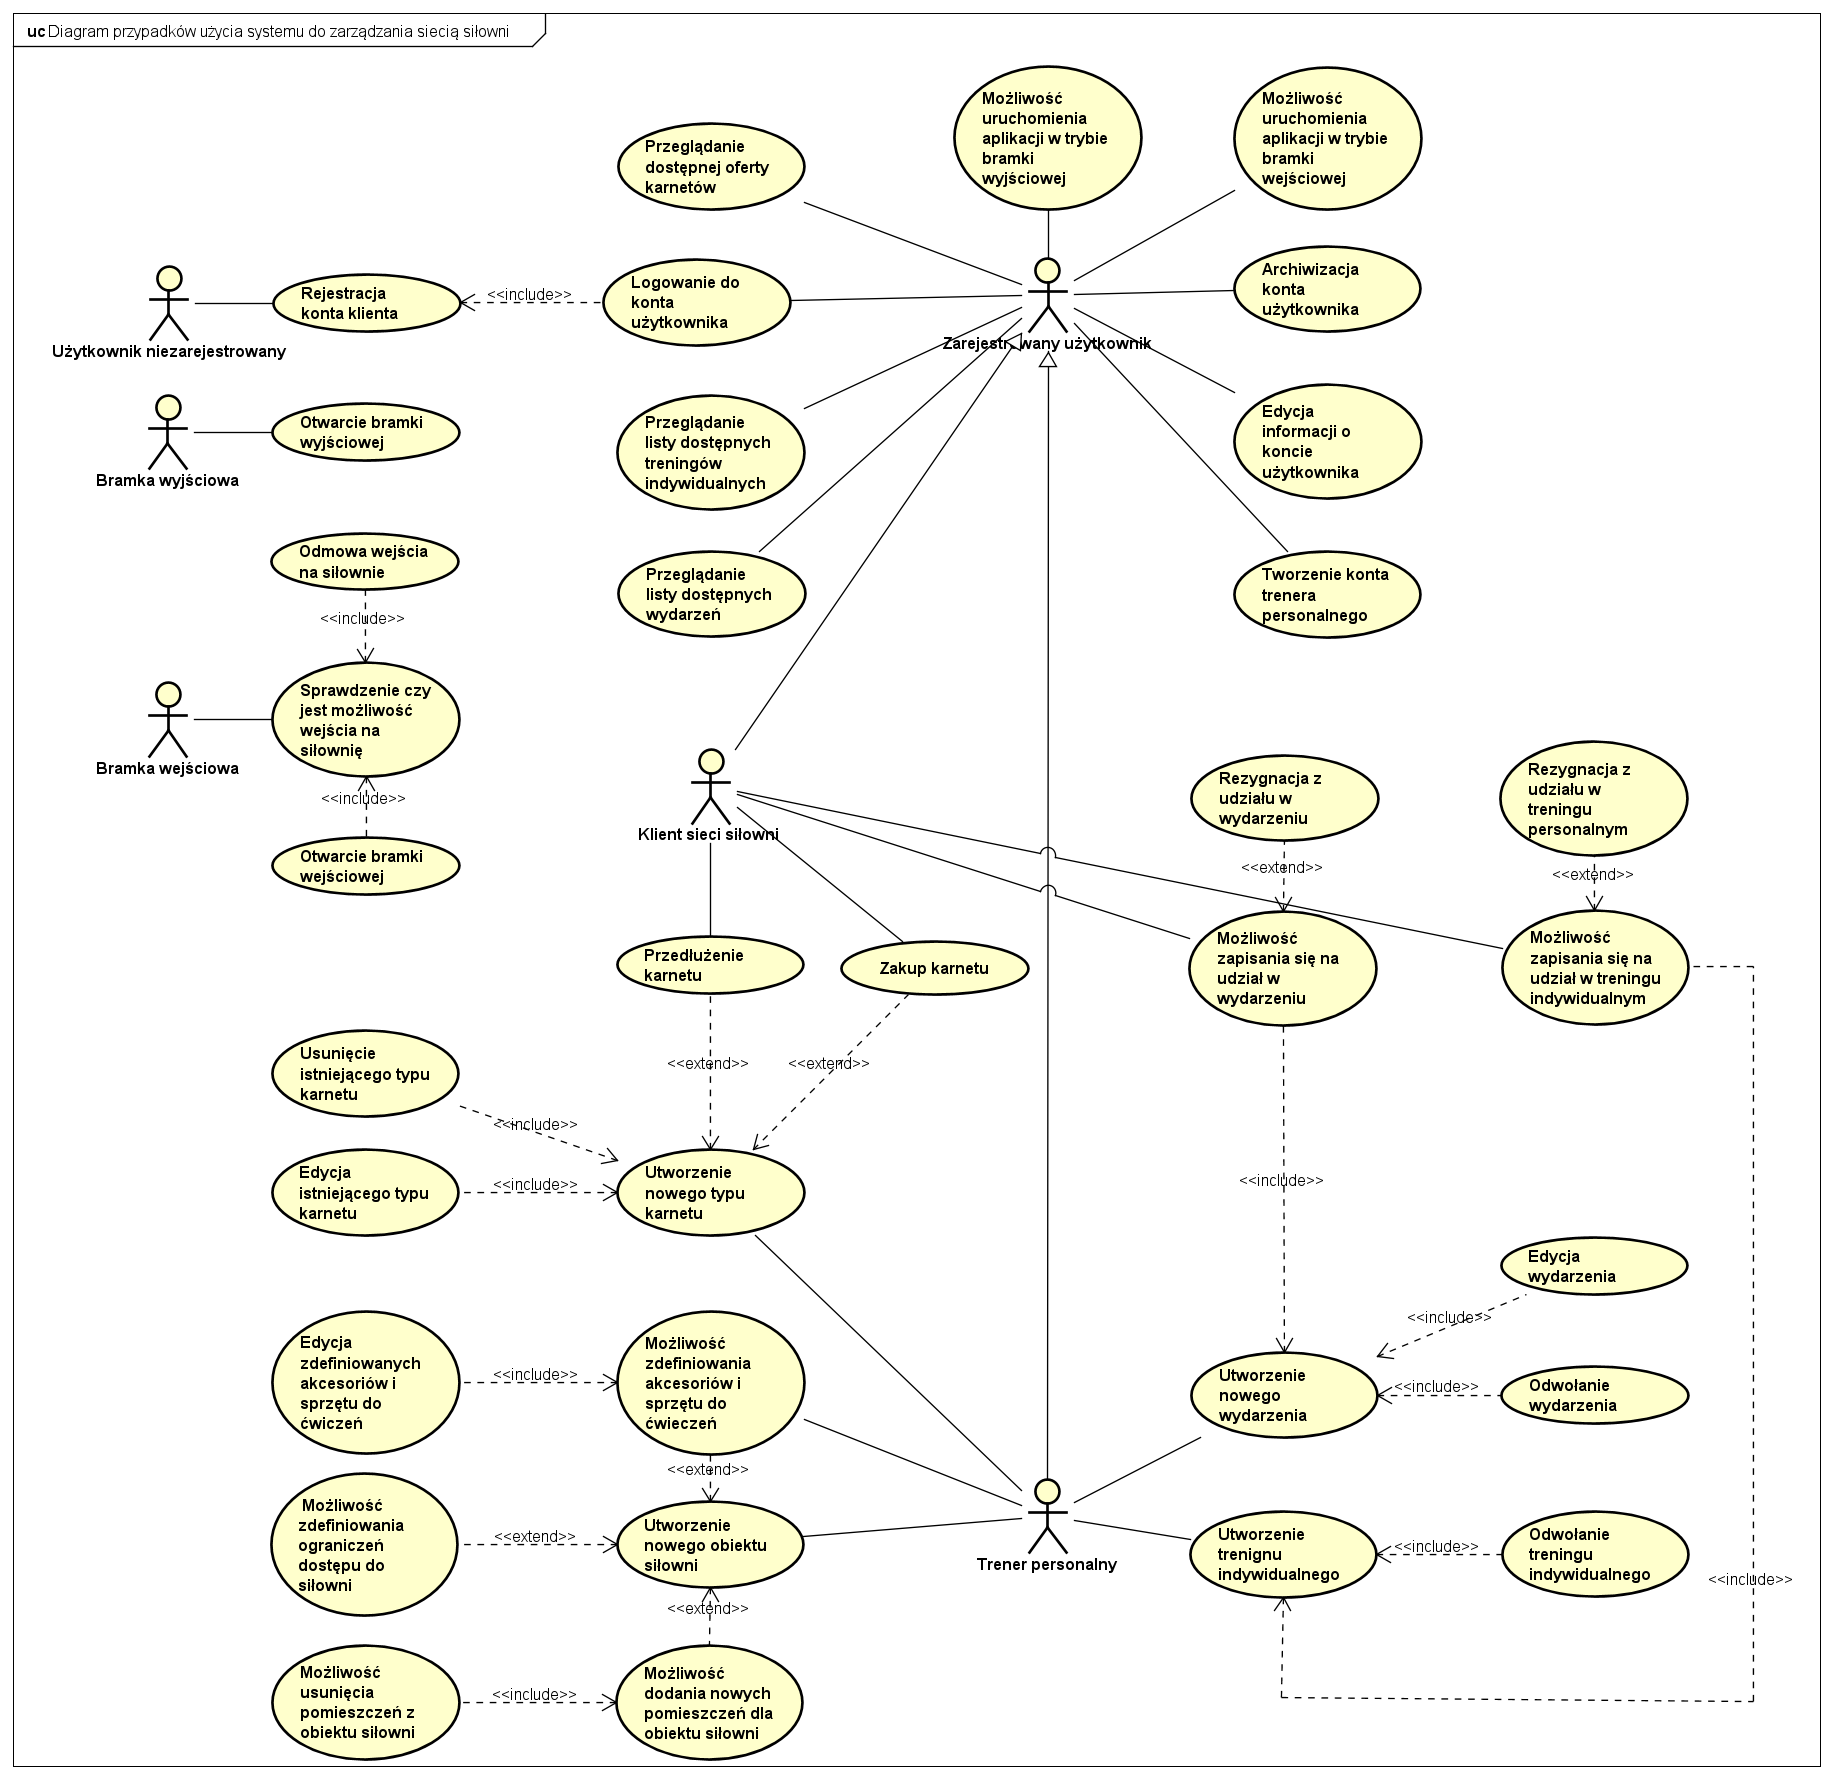
\includegraphics[width=\textwidth]{diagram_przypadków_użycia.png}
	\caption{Diagram przypadków użycia.}
	\label{fig:3}
\end{figure}
	
	\item Narzędzia
	
	Do projektu zostały wykorzystane nowoczesne platformy programistyczne i biblioteki, które posiadają aktualne wsparcie twórców. Wybrano narzędzia w taki sposób, aby pokryć wymagania funkcjonalne projektu oraz wykorzystać technologie, które są aktualnie wykorzystywane w sposób komercyjny.
	
	Językiem programowania użytym do stworzenia części serwerowej został C\# firmy Microsoft. Bliskie podobieństwo do języka Java oraz wiele usprawnień względem niego pozwala na tworzenie oprogramowania przy wykorzystaniu technik programowania obiektowego, funkcyjnego czy generycznego.
	
	Platformą programistyczną warstwy serwerowej został .NET 5, który pozwala na tworzenie aplikacji wieloplatformowych z pomocą języka C\#. Dzięki użyciu następcy .NET Core'a, aplikacja może zostać uruchomiona zarówno na urządzeniach z systemem Microsoft jak i dystrybucjach systemu Linux co pozwala na elastyczność względem wyboru środowiska w którym aplikacja będzie pracować.
	
	Do stworzenia interfejsu REST API została wykorzystana biblioteka ASP.NET Core, która pozwala na dodawanie metod HTTP, które będą następnie konsumowane przez warstwę prezentacji. ASP.NET Core wspiera wykorzystanie kontenerów wstrzykiwania zależności, obsługę autoryzacji przy pomocy żetonu JWT jak i komunikację z wykorzystaniem protokołu HTTPS.
	
	W celu wykorzystania wzorca projektowego CQRS zamiast domyślnego kontenera zależności wykorzystano zewnętrzną bibliotekę Autofac, która udostępnia możliwość wstrzykiwania obiektów oznaczonych atrybutami oraz określanie cyklu życia serwisu przy pomocy znaczników.
	
	Jako bazę danych wykorzystano MongoDB. MongoDB jest dokumentową bazą danych pozwalająca na przechowywanie danych w formacie JSON, który jest formatem czytelnym dla człowieka. Baza danych należy do nierelacyjnych baz danych NoSQL, której głównymi zaletami są: elastyczny schemat bazy, łatwe skalowanie wszerz oraz możliwość tworzenia zaawansowanych zapytań i raportów. Opcja skalowania bazy wszerz jest istotna w systemach, gdzie trzeba zachować ciągłość działania systemu przy rosnącej bazie użytkowników.
	
	Językiem programowania użytym w części wizualnej aplikacji jest język TypeScript zaprojektowany przez firmę Microsoft. W odróżnieniu od języka JavaScript, TypeScript oferuje typowanie w czasie kompilacji, co pozwala na unikanie błędów związanych z niezgodnością typów. Dodanie interfejsów i uogólnień funkcji względem JavaScriptu pozwala na pisanie kodu z wykorzystaniem paradygmatów programowania obiektowego i generycznego.
	
	Do stworzenia interfejsu użytkownika została wykorzystana platforma programistyczna Angular, która pozwala na tworzenie aplikacji internetowych przy wykorzystaniu komponentów wielokrotnego użytku. Cechą charakterystyczną platformy jest natywne wykorzystanie języka TypeScript oraz możliwość tworzenia aplikacji typu SPA.
	
	W celu zminimalizowania czasu potrzebnego na tworzenie komponentów warstwy prezentacji wykorzystano bibliotekę Angular Material z gotowym zestawem rozwiązań. Kontrolki zawarte w bibliotece implementują filozofię Google Material do tworzenia warstw wizualizacji aplikacji internetowych.
	
	W warstwie prezentacji wykorzystano bibliotekę NgXS, która pozwala na wykorzystanie wzorca zarządzania stanem. Rozwiązanie implementuje wzorzec projektowy Redux, którego główną zaletą jest ułatwienie odpluskwiania warstwy prezentacji oraz tworzenie stanów, które są deterministyczne.
	
	\item Metodyka pracy nad projektowaniem i implementacją
	
	Prace rozpoczęto od utworzenia osobnych repozytoriów kodu z uwzględnieniem reprezentowanej warstwy aplikacji. Te warstwy to:
	\begin{itemize}
		\item \textit{Samson.Web.Application} - warstwa serwerowa aplikacji. Zawiera kod, który będzie uruchamiany po stronie serwera.
		\item \textit{Samson.Web.Ui} - warstwa prezentacji aplikacji. Zawiera kod, który będzie uruchamiany na maszynie klienta w celu prezentacji interfejsu użytkownika.
	\end{itemize}

	Następnie podzielono kod warstwy serwerowej na projekty platformy programistycznej .NET. Każdy z projektów został utworzony w taki sposób, aby mógł być zastąpiony w przypadku zmian szczegółów implementacji aplikacji. Podział wygląda następująco:
	\begin{itemize}
		\item \textit{Samson.Web.Application.Api} - projekt zawierający kod kontrolerów platformy ASP.NET, modele wykorzystywane do zapytań HTTP oraz klasy obiektów reprezentujące odpowiedzi serwera na żądania HTTP.
		\item \textit{Samson.Web.Application.Identity} - projekt, który zawiera konfigurację oraz serwisy odpowiedzialne za autoryzację użytkownika.
		\item \textit{Samson.Web.Application.Infrastructure} - projekt posiadający w swojej strukturze utworzone atrybuty, rozszerzenia klas, kod oprogramowania pośredniczącego (ang. \ang Middleware) oraz interfejsy wykorzystywane pomiędzy, różnymi projektami rozwiązania .NET.
		\item \textit{Samson.Web.Application.Persistence} - projekt zawierający kod klas implementujących wzorzec repozytorium. Odpowiada za dodawania i modyfikacje modeli w bazie danych.
		\item \textit{Samson.Web.Application.ReadModels} - projekt platformy .NET implementujący odczyt z bazy danych.
		\item \textit{Samson.Web.Application.UnitTests} - projekt biblioteki NUnit zawierający kod testów jednostkowych.
		\item \textit{Samson.Web.Application.WebHost} - główny projekt aplikacji. Zawiera konfigurację warstwy serwerowej aplikacji
		\item \textit{Samson.Web.Models} - projekt zawierający modele, enumy oraz domenę aplikacji
	\end{itemize}
	
	W następnych krokach implementowano aplikacje tworząc w pierwszej kolejności kontrolery platformy ASP.NET, a w krokach późniejszych dodawano szczegóły implementacji w postaci domeny, warstwy zapisu, warstwy odczytu, modeli. Najważniejsze klasy domenowe zostały uzupełnione testami jednostkowymi w celu zapewnienia poprawności działania. Gdy część serwerowa aplikacji została zakończona, rozpoczęto prace nad warstwą interfejsu użytkownika. Warstwa prezentacji była implementowana w następującej kolejności:
	\begin{enumerate}
		\item Opakowanie komponentów z bibliotek zewnętrznych
		\item Utworzenie widoków i formularzy
		\item Integracja z warstwą serwerową
		\item Dodanie obsługi żetonu JWT w komunikacji z warstwą serwerową
	\end{enumerate}
	
\end{itemize}

\chapter{Specyfikacja zewnętrzna}
Jeśli to Specyfikacja zewnętrzna:
\begin{itemize}
\item  wymagania sprzętowe i programowe
\item  sposób instalacji
\item  sposób aktywacji
\item  kategorie użytkowników
\item  sposób obsługi
\item   administracja systemem
\item  kwestie bezpieczeństwa
\item  przykład działania
\item  scenariusze korzystania z systemu (ilustrowane zrzutami z ekranu lub generowanymi dokumentami)
\end{itemize}

\begin{figure}
\centering

\includegraphics[width=3cm]{logo_pl.jpg}
\caption{Podpis rysunku po rysunkiem.}
\label{fig:2}
\end{figure}


\chapter{Specyfikacja wewnętrzna}
Jeśli to Specyfikacja wewnętrzna:
\begin{itemize}
\item przedstawienie idei
\item architektura systemu
\item opis struktur danych (i organizacji baz danych)
\item komponenty, moduły, biblioteki, przegląd ważniejszych klas (jeśli występują)
\item przegląd ważniejszych algorytmów (jeśli występują)
\item szczegóły implementacji wybranych fragmentów, zastosowane wzorce projektowe
\item diagramy UML
\end{itemize}



Krótka wstawka kodu w linii tekstu jest możliwa, np. \lstinline|descriptor|, a nawet \lstinline|descriptor_gaussian|. 
Dłuższe fragmenty lepiej jest umieszczać jako rysunek, np. kod na rysunku \ref{fig:pseudokod}, a naprawdę długie fragmenty – w załączniku.

\begin{figure}
\centering
\begin{lstlisting}
class descriptor_gaussian : virtual public descriptor
{
   protected:
      /** core of the gaussian fuzzy set */
      double _mean;
      /** fuzzyfication of the gaussian fuzzy set */
      double _stddev;
      
   public:
      /** @param mean core of the set
          @param stddev standard deviation */
      descriptor_gaussian (double mean, double stddev);
      descriptor_gaussian (const descriptor_gaussian & w);
      virtual ~descriptor_gaussian();
      virtual descriptor * clone () const;
      
      /** The method elaborates membership to the gaussian fuzzy set. */
      virtual double getMembership (double x) const;
     
};
\end{lstlisting}
\caption{Klasa \lstinline|descriptor_gaussian|.}
\label{fig:pseudokod}
\end{figure}


\chapter{Weryfikacja i walidacja}
\begin{itemize}
\item sposób testowania w ramach pracy (np. odniesienie do modelu V)
\item organizacja eksperymentów
\item przypadki testowe zakres testowania (pełny/niepełny)
\item wykryte i usunięte błędy
\item opcjonalnie wyniki badań eksperymentalnych
\end{itemize}

\begin{table}
\centering
\caption{Opis tabeli nad nią.}
\label{id:tab:wyniki}
\begin{tabular}{rrrrrrrr}
\toprule
	         &                                     \multicolumn{7}{c}{metoda}                                      \\
	         \cmidrule{2-8}
	         &         &         &        \multicolumn{3}{c}{alg. 3}        & \multicolumn{2}{c}{alg. 4, $\gamma = 2$} \\
	         \cmidrule(r){4-6}\cmidrule(r){7-8}
	$\zeta$ &     alg. 1 &   alg. 2 & $\alpha= 1.5$ & $\alpha= 2$ & $\alpha= 3$ &   $\beta = 0.1$  &   $\beta = -0.1$ \\
\midrule
	       0 &  8.3250 & 1.45305 &       7.5791 &    14.8517 &    20.0028 & 1.16396 &                       1.1365 \\
	       5 &  0.6111 & 2.27126 &       6.9952 &    13.8560 &    18.6064 & 1.18659 &                       1.1630 \\
	      10 & 11.6126 & 2.69218 &       6.2520 &    12.5202 &    16.8278 & 1.23180 &                       1.2045 \\
	      15 &  0.5665 & 2.95046 &       5.7753 &    11.4588 &    15.4837 & 1.25131 &                       1.2614 \\
	      20 & 15.8728 & 3.07225 &       5.3071 &    10.3935 &    13.8738 & 1.25307 &                       1.2217 \\
	      25 &  0.9791 & 3.19034 &       5.4575 &     9.9533 &    13.0721 & 1.27104 &                       1.2640 \\
	      30 &  2.0228 & 3.27474 &       5.7461 &     9.7164 &    12.2637 & 1.33404 &                       1.3209 \\
	      35 & 13.4210 & 3.36086 &       6.6735 &    10.0442 &    12.0270 & 1.35385 &                       1.3059 \\
	      40 & 13.2226 & 3.36420 &       7.7248 &    10.4495 &    12.0379 & 1.34919 &                       1.2768 \\
	      45 & 12.8445 & 3.47436 &       8.5539 &    10.8552 &    12.2773 & 1.42303 &                       1.4362 \\
	      50 & 12.9245 & 3.58228 &       9.2702 &    11.2183 &    12.3990 & 1.40922 &                       1.3724 \\
\bottomrule
\end{tabular}
\end{table}  
 

\chapter{Podsumowanie i wnioski}
\begin{itemize}
\item uzyskane wyniki w świetle postawionych celów i zdefiniowanych wyżej wymagań
\item kierunki ewentualnych danych prac (rozbudowa funkcjonalna …)
\item problemy napotkane w trakcie pracy
\end{itemize}

 
\bibliographystyle{plplain}
\bibliography{bibliografia}
\addcontentsline{toc}{chapter}{Bibliografia}


\begin{appendices}
 

\chapter*{Spis skrótów i symboli}
\addcontentsline{toc}{chapter}{Spis skrótów i symboli}

\begin{itemize}
\item[MVC] model -- widok -- kontroler (ang. \ang{model--view--controller}) 
\item[SPA] jednostronicowa aplikacja internetowa (ang. \ang{Single page application})
\item[CQRS] (ang. \ang{Command and Query Responsibility Segregation})
\item[TS] (ang. \ang{TypeScript]})
\item[JS] (ang. \ang{JavaScript})
\item[REST] (ang. \ang{Representational state transfer})
\item[API] aplikacyjny interfejs programistyczny (ang. \ang{Application programming interface})
\item[JWT] (ang. \ang{JSON Web Token})
\item[JSON] (ang. \ang{JavaScript Object Notation})
\item[HTTP] (ang. \ang{Hypertext Transfer Protocol})
\item[HTTPS] (ang. \ang{Hypertext Transfer Protocol Secure})
\item[NoSQL] nierelacyjna baza danych
\end{itemize}


\chapter*{Źródła}
\addcontentsline{toc}{chapter}{Źródła}

Jeżeli w pracy konieczne jest umieszczenie długich fragmentów kodu źródłowego, należy je przenieść do załącznika.

\begin{lstlisting}
partition fcm_possibilistic::doPartition
                             (const dataset & ds)
{
   try
   {
      if (_nClusters < 1)
         throw std::string ("unknown number of clusters");
      if (_nIterations < 1 and _epsilon < 0)
         throw std::string ("You should set a maximal number of iteration or minimal difference -- epsilon.");
      if (_nIterations > 0 and _epsilon > 0)
         throw std::string ("Both number of iterations and minimal epsilon set -- you should set either number of iterations or minimal epsilon.");
   
      auto mX = ds.getMatrix();
      std::size_t nAttr = ds.getNumberOfAttributes();
      std::size_t nX    = ds.getNumberOfData();
      std::vector<std::vector<double>> mV;
      mU = std::vector<std::vector<double>> (_nClusters);
      for (auto & u : mU)
         u = std::vector<double> (nX);
      randomise(mU);
      normaliseByColumns(mU);
      calculateEtas(_nClusters, nX, ds);
      if (_nIterations > 0)
      {
         for (int iter = 0; iter < _nIterations; iter++)
         {
            mV = calculateClusterCentres(mU, mX);
            mU = modifyPartitionMatrix (mV, mX);
         }
      }
      else if (_epsilon > 0)
      {
         double frob;
         do 
         {
            mV = calculateClusterCentres(mU, mX);
            auto mUnew = modifyPartitionMatrix (mV, mX);
            
            frob = Frobenius_norm_of_difference (mU, mUnew);
            mU = mUnew;
         } while (frob > _epsilon);
      }
      mV = calculateClusterCentres(mU, mX);
      std::vector<std::vector<double>> mS = calculateClusterFuzzification(mU, mV, mX);
      
      partition part;
      for (int c = 0; c < _nClusters; c++)
      {
         cluster cl; 
         for (std::size_t a = 0; a < nAttr; a++)
         {
            descriptor_gaussian d (mV[c][a], mS[c][a]);
            cl.addDescriptor(d);
         }
         part.addCluster(cl);
      }
      return part;
   }
   catch (my_exception & ex)                                  
   {                                                       
      throw my_exception (__FILE__, __FUNCTION__, __LINE__, ex.what()); 
   }                                                          
   catch (std::exception & ex)                                 
   {                                                            
      throw my_exceptionn (__FILE__, __FUNCTION__, __LINE__, ex.what()); 
   }                                                            
   catch (std::string & ex)                                     
   {                                                            
      throw my_exception (__FILE__, __FUNCTION__, __LINE__, ex);        
   }                                                             
   catch (...)                                                   
   {                                                             
      throw my_exception (__FILE__, __FUNCTION__, __LINE__, "unknown expection");       
   }  
}
\end{lstlisting}
 

\chapter*{Zawartość dołączonej płyty}
\addcontentsline{toc}{chapter}{Zawartość dołączonej płyty}

Do pracy dołączona jest płyta CD z~następującą zawartością:
\begin{itemize}
\item praca (źródła \LaTeX owe i końcowa wersja w \texttt{pdf}),
\item źródła programu,
\item dane testowe.
\end{itemize}

\listoffigures
\listoftables
	
\end{appendices}


\end{document}


%% Finis coronat opus.
